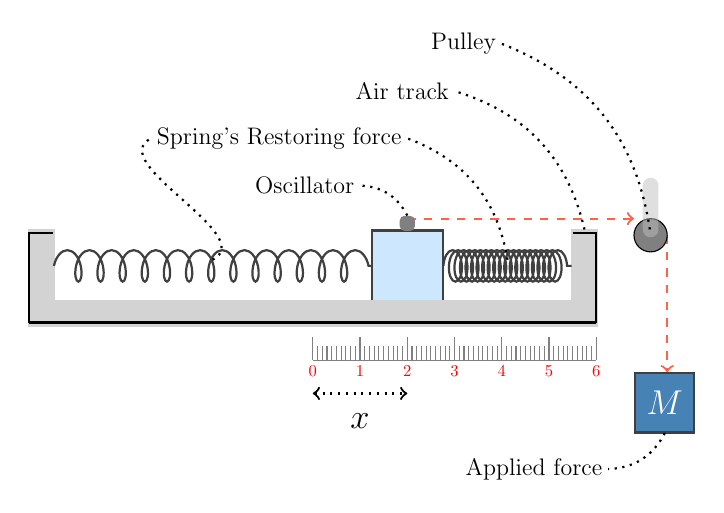
\begin{tikzpicture}[scale=0.6, transform shape]

\tikzstyle{M1}=[rectangle,draw=none,fill=darkgray!50,minimum size=1.5cm]
\tikzstyle{spring}=[darkgray,thick,decorate,decoration={aspect=0.5, segment length=4, amplitude=2mm,coil}]
\tikzstyle{ground}=[fill=LightGray,draw=LightGray,very thick]

% \begin{scope}
% \node[M1,yshift=-0.2cm,xshift=0cm,fill=orange!40](m1a){};
% \node[M1,fill=none,xshift=7.45cm,yshift=-1cm,minimum size=1.25cm](m2){};
% \node[ground,minimum width=12cm,minimum height=0.5cm,yshift=-1.2cm](atrack){};
% % \node[] at (0,2cm) {\Large Equilibrium Position};
% \node[ground,minimum width=0.5cm,minimum height=1.5cm,xshift=-5.75cm,yshift=-0.2cm](LWall){};
% \node[ground,minimum width=0.5cm,minimum height=1.5cm,xshift=5.75cm,yshift=-0.2cm](RWall){};
% \draw [spring] (LWall.east) -- (m1a.west);
% \draw[spring] (m1a.east) -- (RWall.west);
% \end{scope}

\begin{scope}[yshift=-7cm]
        \node [yshift=-1cm, xshift=1cm, anchor=east] (p1) {\Large Oscillator};
        \node [yshift=1cm, anchor=east, xshift=3cm] (p2) {\Large Air track};
        \node [yshift=2cm, anchor=east, xshift=4cm] (p3) {\Large Pulley};
        \node [yshift=-7cm,xshift=6.25cm, anchor=east] (p4) {\Large Applied force};
        \node [anchor=east, xshift=2cm] (p5) {\Large Spring's Restoring force};
  \end{scope}

\begin{scope}[yshift=-9.5cm]
\draw[gray,yshift=-4.5cm] (0,2.3) -- coordinate (x axis mid) (6,2.3);
\foreach \x in {0,...,6}
     		\draw[yshift=-4.5cm,gray,text=red] (\x,2.8) -- (\x,2.3)
			node[anchor=north] {\x};
\foreach \xx in {1,...,60}
            \draw[yshift=-4.5cm,gray] (\xx/10,2.6) -- (\xx/10,2.3){};

\draw[<->,thick,yshift=-5.9cm,dotted] (0,3) -- node[yshift=-.3cm,below] {\huge $x$} ++(2,0);
\draw[->,Tomato,thick, dashed] (2,0.8)--(6.8,0.8){};
\draw[->,Tomato,thick, dashed,yshift=-10pt,xshift=10pt] (7.15,0.8)--(7.15,-2.1){};
\filldraw [fill=gray,yshift=-10pt] (7.15,0.8) circle (10pt) node (pul) {};

\node[M1,yshift=-0.2cm,xshift=2cm,fill=DodgerBlue!22,draw=darkgray,thick](m1){};
\node[M1,text=White,xshift=7.45cm,yshift=-3.1cm,minimum size=1.25cm,draw=darkgray, thick, fill=SteelBlue](m2){\huge $\bm M$};
\node[rectangle,rounded corners=0.4ex,draw=none,fill=gray,minimum size=0.32cm,yshift=0.7cm,xshift=2cm](p1x){};
\node[ground,minimum width=12cm,minimum height=0.5cm,yshift=-1.2cm,text=white](atrackb){};
\draw[thick] (-6,-1.4) -- (6,-1.4);
% \node[] at (0,-2) {\huge Displacement $x$, caused by force = $mg$};
\node[ground,minimum width=0.5cm,minimum height=1.5cm,xshift=-5.75cm,yshift=-0.2cm](LWallb){};
\draw[thick] (-6,-1.4) -- (-6,0.5) -- (-5.5,0.5);
\node[ground,minimum width=0.5cm,minimum height=1.5cm,xshift=5.75cm,yshift=-0.2cm](RWallb){};
\draw[thick] (6,-1.4) -- (6,0.5) -- (5.5,0.5);
\draw[line width=2mm, line cap=round, lightgray, opacity=0.5] (7.15,1.5) -- (pul.north);
\draw [spring,segment length=8] (LWallb.east) -- (m1.west) node[midway, above](s1){};
\draw[spring, segment length=2](m1.east) -- (RWallb.west) node[midway, above](s2){};
\end{scope}

        \path[thick] (p1x.north) edge [dotted, bend right] (p1.east);
        \path[thick] (pul) edge [dotted, bend right] (p3.east);
        \path[thick] (s1.center) edge [dotted,bend left=10, in=90,out=-90] (p5.west);
        \path[thick] (s2.center) edge [dotted,bend right] (p5.east);
        \path[thick] (m2.south) edge [dotted,bend left] (p4.east);
        \path[thick] (RWallb.north) edge [dotted,bend right] (p2.east);

\end{tikzpicture}